\documentclass[11pt]{article}
\usepackage[margin=1in]{geometry}
\usepackage{graphicx, booktabs, hyperref, xcolor, parskip, amsmath}

\begin{document}

\begin{center}
{\Large \textbf{Experiment Results:\\Costly Punishment in the Repeated Prisoner's Dilemma\\with Concordia Agents}}\\[0.5em]
{\large February 2026 \quad $\cdot$ \quad Status: Post-analysis}
\end{center}

%% --- 1. RESEARCH QUESTION ---
\section*{Research Question}

Does the availability of costly punishment increase cooperation among LLM-based agents in a finitely repeated Prisoner's Dilemma?

In the baseline experiment (\texttt{pd\_concordia}, post-fix), Concordia \texttt{RationalEntity} agents achieved $\sim$60\% average cooperation with only 20\% of games reaching full mutual cooperation. The remaining 80\% featured early defection with no recovery. Costly punishment---a mechanism well-established in the behavioral economics literature (Fehr \& G\"achter, 2000, 2002)---allows players to reduce a defector's earnings at a personal cost, creating incentives for cooperation even in finite games.

\textbf{Hypothesis:} The availability of costly punishment (pay \$1 to reduce the other player's earnings by \$3) increases full cooperation from 20\% to $>$50\% and average cooperation from 60\% to $>$80\%.

%% --- 2. EXPERIMENTAL DESIGN ---
\section*{Experimental Design}

\textbf{Game:} Repeated Prisoner's Dilemma, 10 rounds, 2 symmetric players. Each round has two stages:

\begin{enumerate}
\item \textbf{PD stage:} Both players simultaneously choose COOPERATE or DEFECT. Payoffs: CC=\$3/\$3, CD=\$0/\$5, DC=\$5/\$0, DD=\$1/\$1.
\item \textbf{Punishment stage:} After observing the PD outcome, both players simultaneously choose PUNISH or NO\_PUNISH. Punishing costs \$1 and reduces the target's round earnings by \$3. Round earnings can go negative.
\end{enumerate}

\textbf{Conditions:}
\begin{center}
\begin{tabular}{lll}
\toprule
Condition & Punishment available? & N \\
\midrule
Baseline (\texttt{pd\_concordia}) & No & 30 \\
Punishment (\texttt{pd\_concordia\_punish}) & Yes & 30 \\
\bottomrule
\end{tabular}
\end{center}

\textbf{Agent architecture:} Concordia \texttt{RationalEntity} prefab. Model: \texttt{gpt-4o-mini}. Randomized act-order each round within each stage. Role-relative observations (``You'' / ``the other player''). Both conditions use the same architecture; the only difference is the presence of the punishment stage.

\textbf{Seeds:} Baseline: seed 43. Punishment: seed 42.

%% --- 3. DATA OVERVIEW ---
\section*{Data Overview}

\textbf{Sample:} 60 simulations (30 per condition), 600 total PD rounds. All sessions completed all 10 rounds. Zero invalid actions across all rounds in both conditions.

\textbf{Summary statistics:}

\begin{center}
\begin{tabular}{l rr rr}
\toprule
 & \multicolumn{2}{c}{Baseline} & \multicolumn{2}{c}{Punishment} \\
Metric & Mean & SD & Mean & SD \\
\midrule
A earnings (\$) & 22.9 & 7.3 & 29.6 & 2.2 \\
B earnings (\$) & 22.6 & 7.5 & 29.4 & 3.3 \\
Joint earnings (\$) & 45.5 & 12.7 & 59.0 & 5.5 \\
Efficiency & 0.76 & 0.21 & 0.98 & 0.09 \\
A cooperation rate & 0.59 & 0.37 & 0.99 & 0.05 \\
B cooperation rate & 0.60 & 0.37 & 0.99 & 0.05 \\
Mutual coop rounds & 5.0 & 4.5 & 9.9 & 0.7 \\
Full coop games & \multicolumn{2}{c}{6/30 (20\%)} & \multicolumn{2}{c}{29/30 (97\%)} \\
\midrule
A punishment rate & --- & --- & 0.013 & 0.073 \\
B punishment rate & --- & --- & 0.003 & 0.018 \\
Punishments/game & --- & --- & 0.17 & 0.91 \\
\bottomrule
\end{tabular}
\end{center}

%% --- 4. RESULTS ---
\section*{Results}

\subsection*{Primary Outcome: Cooperation Rate}

The punishment condition produced near-universal cooperation. Average cooperation increased from 59\% to 99\% ($t(58) = -5.94$, $p < 0.0001$; Mann-Whitney $U = 102$, $p < 0.0001$). Full cooperation games increased from 20\% (6/30) to 97\% (29/30) (Fisher's exact $p < 0.0001$).

Both predictions were confirmed: full cooperation exceeded 50\% (observed: 97\%) and mean cooperation exceeded 80\% (observed: 99\%).

\begin{figure}[ht]
\centering
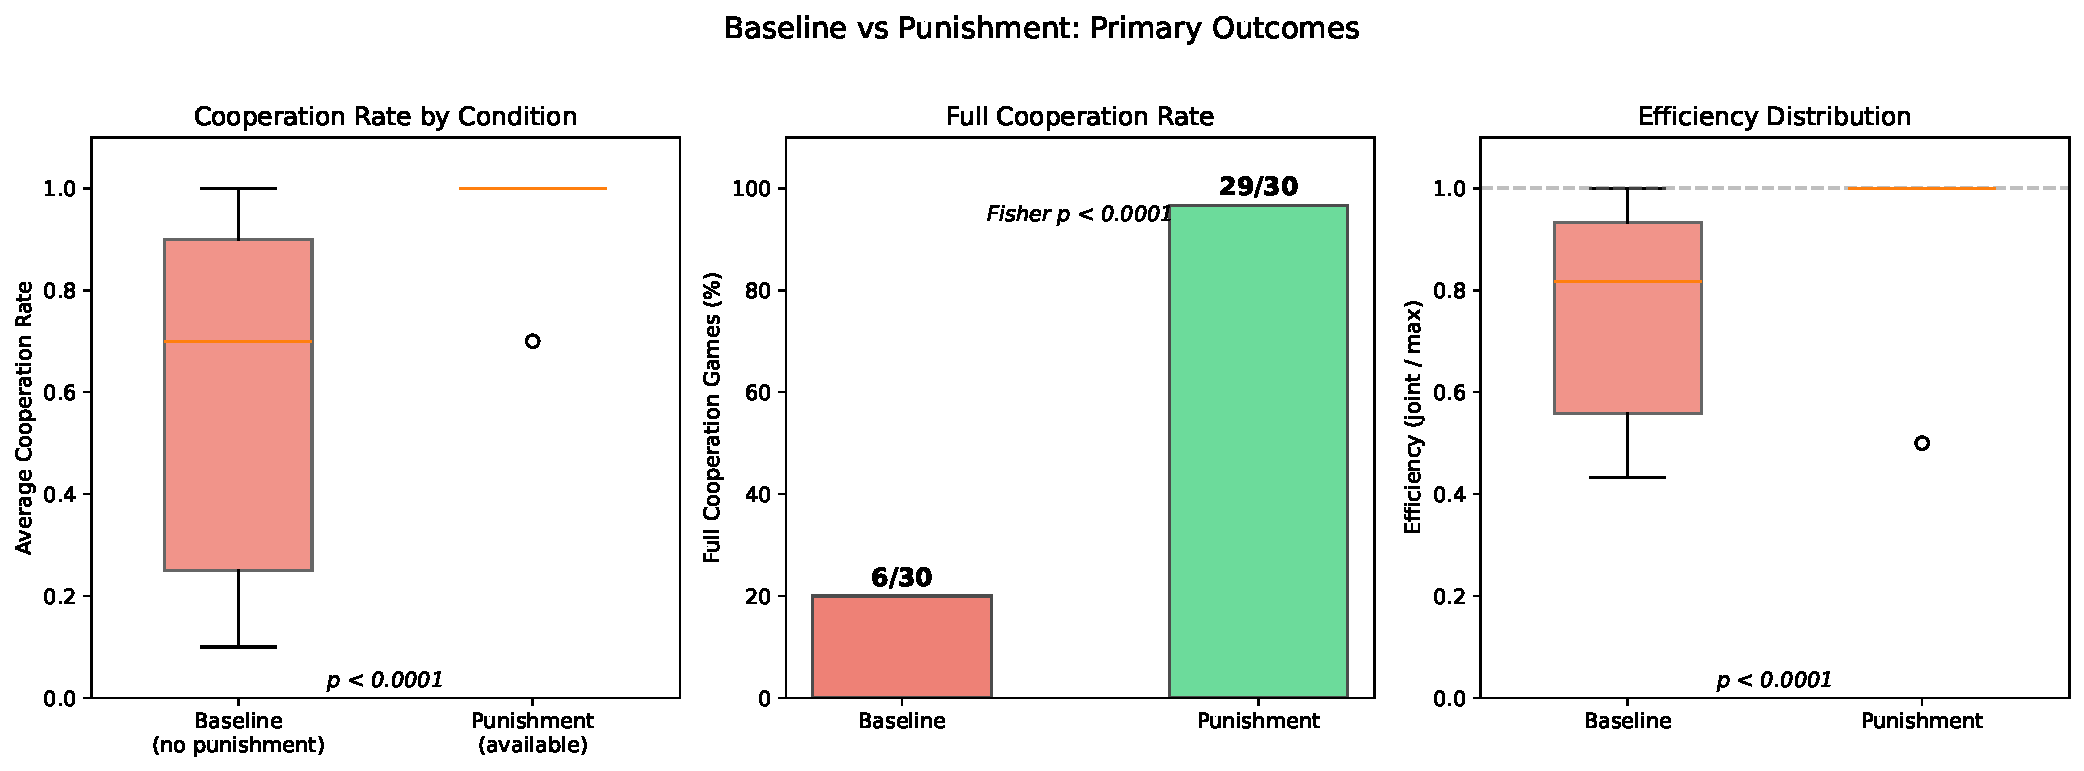
\includegraphics[width=0.95\textwidth]{plots/results_main_outcomes.pdf}
\caption{Primary outcomes by condition. Left: Average cooperation rate (box plot). Center: Full cooperation games (\%). Right: Efficiency. All three metrics are dramatically higher in the punishment condition ($p < 0.0001$).}
\end{figure}

\subsection*{Round-by-Round Dynamics}

The punishment condition shows near-ceiling cooperation in every round (97--100\%). The baseline shows the previously documented pattern of $\sim$40--67\% cooperation with no endgame effect. The largest gap is in Round 1: baseline A cooperates 40\% vs.\ punishment A cooperates 100\%.

\begin{figure}[ht]
\centering
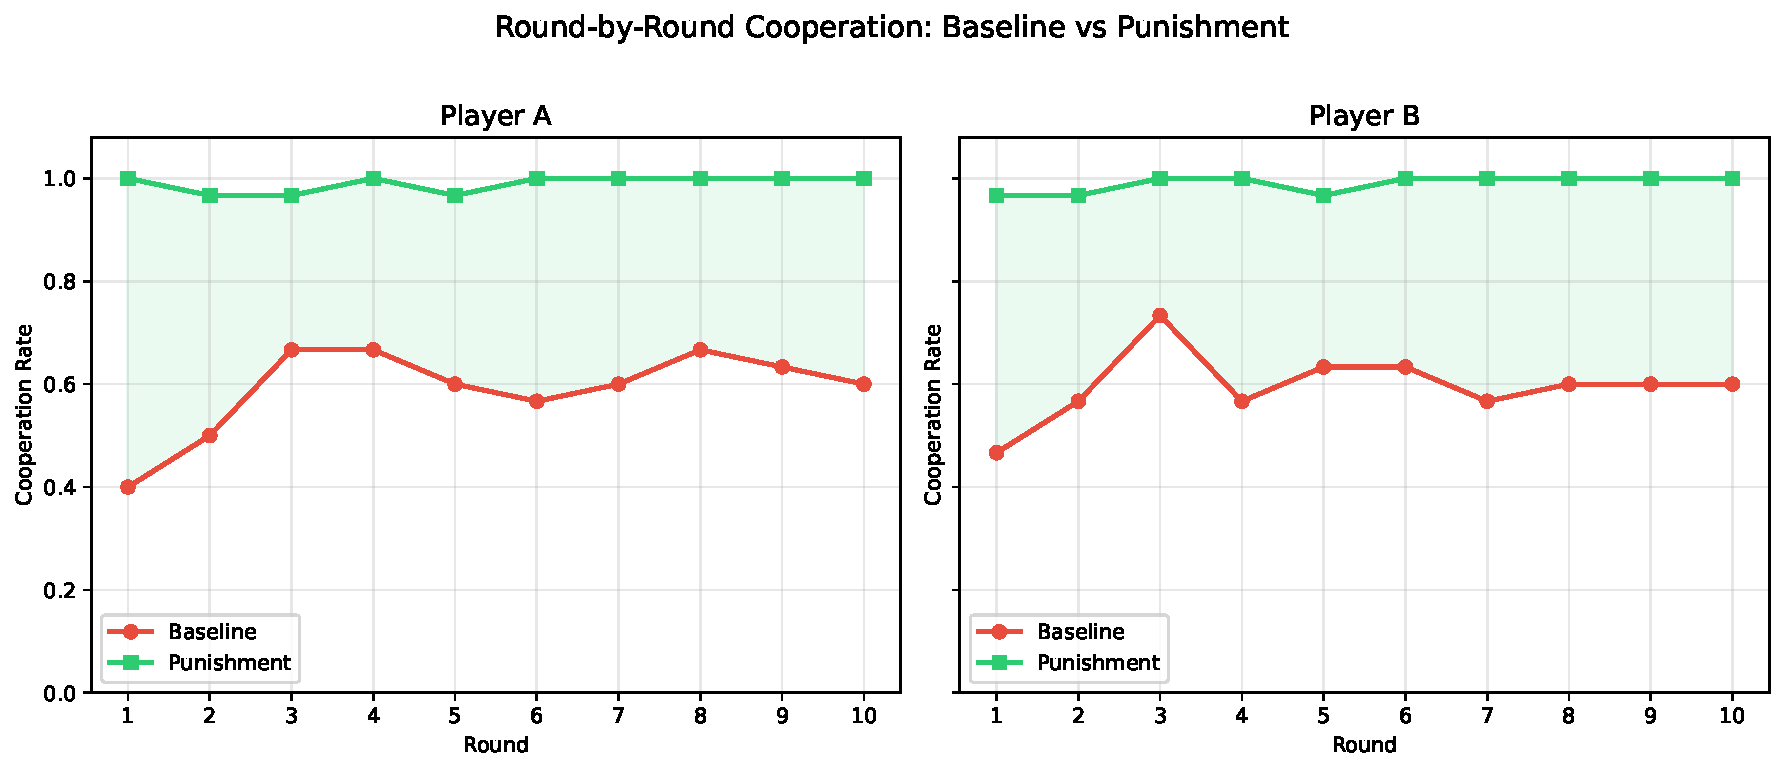
\includegraphics[width=0.95\textwidth]{plots/results_round_by_round.pdf}
\caption{Round-by-round cooperation rates. The punishment condition (green) maintains near-ceiling cooperation throughout. The baseline (red) fluctuates between 40--70\%.}
\end{figure}

\subsection*{Earnings and Efficiency}

Joint earnings increased from \$45.5 to \$59.0 ($t = -5.33$, $p < 0.0001$). Efficiency rose from 76\% to 98\%. Earnings are symmetric in both conditions: the A$-$B gap is $+$\$0.3 (baseline, $p = 0.81$) and $+$\$0.2 (punishment, $p = 0.33$).

\begin{figure}[ht]
\centering

\includegraphics[width=0.95\textwidth]{plots/results_earnings.pdf}
\caption{Left: A vs.\ B earnings scatter (punishment games cluster at \$30/\$30; baseline is dispersed). Right: Joint earnings distribution (punishment concentrated at \$60; baseline spread from \$26--\$60).}
\end{figure}

\subsection*{Punishment Usage: The Critical Detail}

Despite the dramatic cooperation increase, \textbf{punishment was almost never used}. Only 1 of 30 games (simulation 27) featured any punishment at all. In that game:

\begin{enumerate}
\item Round 1: B defected, A cooperated. A then punished B (A earned $-$\$1, B earned \$2).
\item Rounds 2--4: Mixed play with A punishing aggressively (4 punishments in 5 rounds).
\item Rounds 5--10: Stable mutual cooperation with no punishment.
\item Final outcome: A=\$18, B=\$12 (punishment was costly to both).
\end{enumerate}

The remaining 29 games achieved perfect cooperation with zero punishment. This means the \emph{threat} of punishment, not its actual use, drove the cooperation increase. Agents cooperated preemptively because the punishment mechanism was described in their goal string.

\begin{figure}[ht]
\centering
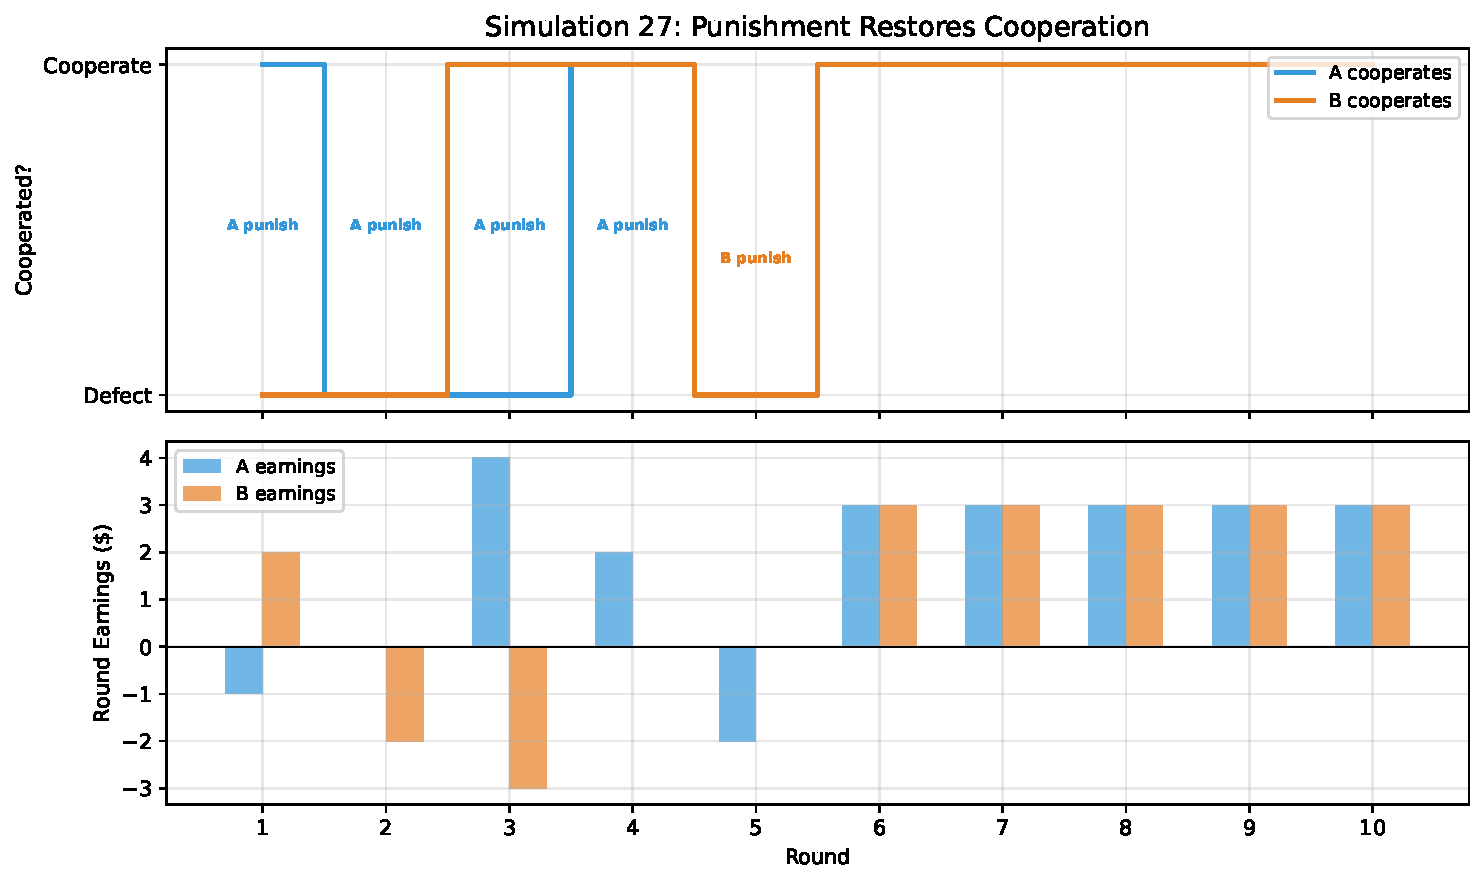
\includegraphics[width=0.95\textwidth]{plots/results_sim27_detail.pdf}
\caption{Simulation 27: The only game with punishment. Top: PD choices (A punishes B after defection). Bottom: Round earnings (punishment creates negative earnings in early rounds before cooperation stabilizes).}
\end{figure}

%% --- 5. EVALUATION ---
\section*{Evaluation}

\subsection*{Did We Learn Something Interesting?}

\textbf{Partially --- the result is clear but the mechanism is different from what was hypothesized.}

\begin{enumerate}
\item \textbf{The punishment condition dramatically increased cooperation} (20\% $\to$ 97\% full cooperation, $p < 0.0001$). This is the largest treatment effect observed in this project. \textbf{CONFIRMED.}

\item \textbf{But the mechanism is not punishment-as-deterrent --- it is prompt-as-framing.} In human experiments, costly punishment works because defectors \emph{experience} punishment and adjust behavior. Here, 29/30 games had zero punishment. The agents cooperated because their goal string \emph{mentioned} punishment as a possibility, which appears to have shifted the LLM's prior toward cooperation. This is a \textbf{framing effect}, not a strategic response to punishment incentives.

\item \textbf{The one game with actual punishment (sim 27) is consistent with deterrence theory:} A punished B's defection, and B eventually cooperated. But $N = 1$ is anecdotal, not evidence.
\end{enumerate}

\textbf{Diagnosis: the treatment is confounded.} Adding the punishment stage changed \emph{two things} simultaneously: (a) the strategic structure (punishment is available) and (b) the goal string (which now describes punishment mechanics). We cannot distinguish whether cooperation increased because agents understood the punishment threat and cooperated strategically, or because the longer/richer goal string simply primed cooperative behavior.

\subsection*{Limitations}

\begin{itemize}
\item \textbf{Framing confound:} The punishment condition's goal string is longer and describes a more complex game. The extra text about punishment may function as a cooperation prime, independent of the actual punishment mechanism. A control with the same goal string length but no punishment mechanic would disentangle this.
\item \textbf{Ceiling effect:} 97\% full cooperation leaves no room to detect moderators or heterogeneity. The effect is so large that it may be an artifact.
\item \textbf{Single model:} \texttt{gpt-4o-mini} may be especially susceptible to framing effects. Other models may show different sensitivity.
\item \textbf{No punishment equilibrium path:} With 29/30 games at full cooperation, we cannot study \emph{how} agents use punishment because they never need to. The game needs to be redesigned to create more defection opportunities.
\end{itemize}

%% --- 6. NEXT EXPERIMENT ---
\section*{Next Experiment}

\textbf{Recommended archetype: REFINE}

The key unresolved question is whether the cooperation increase is a \textbf{strategic response to punishment availability} or a \textbf{framing/priming effect from the goal string}. This must be disentangled before the result is interpretable.

\textbf{Proposed experiment: Framing Control}

Three conditions:
\begin{enumerate}
\item \textbf{Baseline:} Standard PD, short goal string (current \texttt{pd\_concordia}).
\item \textbf{Punishment:} PD + punishment stage (current \texttt{pd\_concordia\_punish}).
\item \textbf{Framing control:} Standard PD (no punishment mechanic) but with a goal string that \emph{describes} punishment as a hypothetical possibility that is ``not available in this version.'' This matches the punishment condition's goal string length and complexity without adding the actual mechanism.
\end{enumerate}

\textbf{Predictions:}
\begin{itemize}
\item If \textbf{strategic deterrence} drives cooperation: Punishment $>$ Framing control $\approx$ Baseline.
\item If \textbf{framing/priming} drives cooperation: Punishment $\approx$ Framing control $>$ Baseline.
\end{itemize}

\textbf{Alternative approach:} Instead of a framing control, engineer more defection in the punishment condition by adding a ``temptation bonus'' (e.g., increase the defection payoff from \$5 to \$8) to create scenarios where agents actually need to use punishment. This would let us observe punishment dynamics directly.

\textbf{Next step:} Run \texttt{/create-concordia-game} for the framing-control condition, then run all three conditions and compare.

\subsection*{Prior Experiment Context (Machine-Readable)}
\begin{verbatim}
prior_hypothesis: Costly punishment availability increases cooperation
  from 20% full-coop to >50% by deterring defection
verdict: PARTIALLY
diagnosis: DESIGN
key_finding: Punishment increased full cooperation from 20% to 97%
  (p<0.0001), but punishment was never used in 29/30 games,
  suggesting framing/priming rather than strategic deterrence
key_statistic: full_coop_baseline=20%, full_coop_punishment=97%,
  punishment_used_in=1/30_games, total_punishments=5/600_opportunities
dag_variables: X=punishment_availability, M=strategic_deterrence_OR_framing,
  Y=cooperation_rate, Z=payoff_structure
testable_implications_results: full_coop>50%=CONFIRMED,
  mean_coop>80%=CONFIRMED, punishment_used_as_deterrent=UNCLEAR(N=1),
  mechanism_is_strategic=UNCONFIRMED
next_archetype: REFINE
proposed_changes: Add framing-control condition (same goal string
  length/complexity but no actual punishment mechanism) to
  disentangle strategic deterrence from goal-string priming
next_hypothesis_sketch: The cooperation increase is driven by
  goal-string framing (mentioning punishment primes cooperation)
  rather than strategic response to punishment availability
\end{verbatim}

\end{document}
